
\myparagraph{Прямое и обратное преобразования Фурье}

Любой сигнал и любое изображение, как частный случай сигнала, могут быть описаны в виде функций от одной или нескольких переменных. Так, изображение $I$ может быть описано как функция от двух переменных \eqref{ip:3:image}:
\begin{gather}
	\label{ip:3:image} f(x, y) \in \mathbb{R} ~;~ x \in [0 ~;~ w] ~;~ y \in [0 ~;~ h] ~;~w, h \in \mathbb{N} \\
	\notag f(x, y) = 0 ~;~ x \notin [0 ~;~ w] ~;~ y \notin [0 ~;~ h],
\end{gather}

где:

\begin{itemize}

	\item $w$, $h$ - соответственно, количество строк и столбцов в изображении;
	\item $x$, $y$ - координаты пикселя в изображении.

\end{itemize}

Как правило, любое изображение является дискретным - то есть состоит из простых точек (<<пикселей>>) и не описывает способ расчета значения функции $f(x, y)$ на отрезках между соседними пикселями. Дискретность изображения суть есть требование к функции $f(x, y)$ принимать только целые аргументы: $x \in \mathbb{Z}^+ ~;~ y \in \mathbb{Z}^+$. Дискретность изображения в некоторых случаях затрудняет его анализ, поэтому ее удобно игнорировать путем ввода некоторого способа расчета функции $f(x, y)$ для не целых аргументов.

Функция $f(x, y)$, очевидно, является объектом части пространств $L^p$. Пространство $L^p$ суть есть пространство измеримых функций, $p$-я степень которых интегрируема, при условии, что $p \ge 1$. Как минимум, $f(x, y) \in L^1$. Как и любое пространство, пространство $L^1$ располагает бесконечно большим количеством базисов. Идея некоторых подходов к анализу изображения (в том числе и идея частотного анализа изображения) состоит в расчете координат функции $f(x, y)$ в пространстве $L^1$ по заданному базису, применении тех или иных преобразований к полученному вектору координат и расчете линейной комбинации функции, составляющих базис, по вектору координат с получением в результате преобразованной функции $f^*(x, y)$.

Изучением возможных базисов пространства $L^1$ занимаются различные разделы математики - теория вейвлет - анализа, теория анализа Фурье, теория преобразования Карунена - Лоева и прочие. В настоящей лабораторной работе рассматривается наиболее известный и популярный базис - базис Фурье (базис, образованный экспоненциальными функциями).

Расчет координат функции $f(x, y)$ в базисе Фурье выполняется с помощью прямого двумерного преобразования Фурье \eqref{ip:3:fn}. В случае дискретной функции $f(x, y)$ (в случае реального изображения) преобразование выполняется по формуле \eqref{ip:3:dfn}, которая получается из \eqref{ip:3:fn} заменой интегрирования суммированием (которым интегрирование, с дискретной точки зрения, и является):
\begin{gather}
	\label{ip:3:fn} F(u, v) = \int\limits_{- \infty}^{\infty} \int\limits_{- \infty}^{\infty} f(x, y) e^{-i 2 \pi (ux + vy)} dx dy \\
	\label{ip:3:dfn} F(u, v) = \dfrac{1}{wh} \sum\limits_{x = 0}^{w - 1} \sum\limits_{y = 0}^{h - 1} f(x, y) e^{-i 2 \pi (ux / w + vy / h)},
\end{gather}

где $u$, $v$ суть есть координаты компоненты вектора координат $F$ функции $f(x, y)$ в базисе Фурье.

С физической точки зрения, преобразование Фурье является способом анализа распределения сигнала по частотому диапазону. Координаты $u$ и $v$ являются в такой интерпретации преобразования Фурье номерами частот, а компоненты вектора $F$ представляют из себя оценку амплитуды $(u, v)$-ой частотной составляющей сигнала (изображения).

Линейная комбинация экспоненциальных функции по вектору $F$ суть есть обратное двумерное преобразование Фурье, вычисляемое по формулам \eqref{ip:3:ofn} (непрерывный сигнал) и \eqref{ip:3:odfn} (дискретный сигнал).
\begin{gather}
	\label{ip:3:ofn} f(x, y) = \int\limits_{- \infty}^{\infty} \int\limits_{- \infty}^{\infty} F(x, y) e ^{i 2 \pi (ux + vy)} dx dy \\
	\label{ip:3:odfn} f(x, y) = \sum\limits_{u = 0}^{w - 1} \sum\limits_{v = 0}^{h - 1} F(x, y) e ^{i 2 \pi (ux / w + vy / h)}.
\end{gather}

Библиотека OpenCV предоставляет разнообразный функционал для частотного анализа изображений.

Для выполнения прямого дискретного двумерного преобразования Фурье над исходным изображением можно воспользоваться функцией \verb|dft()|, прототип которой приведен в листинге \ref{listing:ip:3:dft}.

\mylistingbegin{ip:3:dft}{Прямое преобразование Фурье над исходным изображением с помощью функции dft()}
\begin{lstlisting}

void dft(Mat I, Mat & R, int flags);

\end{lstlisting}
\mylistingend

Функция \verb|dft()| обладает следующими параметрами:

\begin{itemize}

	\item \verb|I| - преобразуемое двуканальное изображение.

	Первый канал изображения $I$ суть есть канал исходного изображения, второй канал изображения $I$ должен быть заполнен нулями. Оба канала должны быть вещественными.

	В листинге \ref{listing:ip:3:iinit} приведен способ инициализации изображения $I$.

\mylistingbegin{ip:3:iinit}{Инициализация преобразуемого двуканального изображения}
\begin{lstlisting}

Mat I;
vector<Mat> ch_I = {Mat_<float>(ch[i]), Mat::zeros(size, CV_32F)};

merge(ch_I, I);

\end{lstlisting}
\mylistingend

	В листинге \ref{listing:ip:3:iinit} используются следующие переменные и объекты:

	\begin{itemize}

		\item \verb|ch| - массив каналов исходного изображения;
		\item \verb|i| - номер преобразуемого канала;
		\item \verb|size| - объект класса \verb|Size|, содержащий информацию о размере исходного изображения.

	\end{itemize}

	Функция \verb|merge()| создает двуканальное изображение \verb|I|, первым и вторым каналами которого становятся соответствующие элементы массива \verb|ch_I|;

	\item \verb|R| - результирующее изображение с вещественными каналами;

	\item \verb|flags| - маска флагов.

	Маска флагов составляется путем применения операции побитового ИЛИ над значениями одной или нескольких специальных констант компилятора. В настоящей лабораторной работе рекомендуется указывать единственную константу компилятора: \linebreak \verb|DFT_COMPLEX_OUTPUT|, что предписывает библиотеке сохранить результат преобразования в двуканальном изображении \verb|R|, каналы которого будут содержать соответственно вещественные и комплексные части частотных характеристик.

\end{itemize}

Необходимо помнить, что функция \verb|dft()| центрирует спектр частот, домножая исходное изображение на $(-1)^{x + y}$ - результирующее изображение \verb|R| является симметричным по горизонтали и вертикали, причем постоянная составляющая исходного изображения находится в центре изображения \verb|R|, а по краям данного изображения находятся высокочастотные составляющие исходного изображения.

Также важно отметить тот факт, что функция \verb|dft()| без указания специального флага не масштабирует значения пикселей результирующего вещественного изображения, поэтому перед выводом результирующего изображения значения его пикселей необходимо отмасштабировать в диапазон $[0 ~;~ 1]$. Масштабирование значений пикселей некоторого одноканального вещественного изображения \verb|T| можно выполнить с помощью последовательности действий, приведенных в листинге \ref{listing:ip:3:scale}.

\mylistingbegin{ip:3:scale}{Масштабирование вещественного изображения}
\begin{lstlisting}

normalize(T, T, 0, 1, NORM_MINMAX);
T *= SCALE;

\end{lstlisting}
\mylistingend

В листинге \ref{listing:ip:3:scale} функция \verb|normalize()| масштабирует значения пикселей изображения \verb|T| в диапазон $[0 ~;~ 1]$, после чего изображение \verb|T| домножается на некоторый масштабирующий коэффициент, что необходимо в тех случаях, когда лишь малая часть пикселей приходится на большую часть диапазона $[0 ~;~ 1]$ - в общем случае, белым цветом выводятся те пиксели, значение которых равно или привосходит единицу, поэтому целесообразным представляется домножение, делающее неразличимыми при выводе малую часть пикселей, лежащих в большей части диапазона $[0 ~;~ 1]$ и часть пикселей из меньшей части диапазона, но при этом увеличивающее контраст между пикселями из меньшей части диапазона.

При необходимости вывода на экран результатов преобразования Фурье чаще всего выполняют вывод не вещественных и комплексных составляющих преобразования, но вывод амплитудной или фазовой характеристик преобразования.

Для расчета амплитудной составляющей преобразования можно воспользоваться функцией \verb|magnitude()|, прототип которой приведен в листинге \ref{listing:ip:3:magn}.

\mylistingbegin{ip:3:magn}{Расчет амплитудной составляющей преобразования с помощью функции magnitude()}
\begin{lstlisting}

void magnitude(Mat R, Mat C, Mat & A);

\end{lstlisting}
\mylistingend

Функция \verb|magnitude()| расчитывает амплитудную составляющую \verb|A| преобразования по его вещественной \verb|R| и комплексной \verb|C| составляющим.

Для расчета фазовой составляющей преобразования можно воспользоваться функцией \verb|phase()|, прототип которой приведен в листинге \ref{listing:ip:3:phase}.

\mylistingbegin{ip:3:phase}{Расчет фазовой составляющей преобразования с помощью функции phase()}
\begin{lstlisting}

void phase(Mat R, Mat C, Mat & phase);

\end{lstlisting}
\mylistingend

В случае $r \in R ~;~ c \in C ~;~ r = c = 0$ фазовая составляющая условно принимается равной нулю.

Обратное дискретное двумерное преобразование Фурье реализовано в виде функции \verb|idft()|, прототип которой приведен в листинге \ref{listing:ip:3:idft}.

\mylistingbegin{ip:3:idft}{Обратное дискретное двумерное преобразование Фурье с помощью функции idft()}
\begin{lstlisting}

void idft(Mat R, Mat & IS, int flags);

\end{lstlisting}
\mylistingend

Функция \verb|idft()| обладает следующими параметрами:

\begin{itemize}

	\item \verb|R| - преобразуемое двуканальное вещественное изображение;
	\item \verb|IS| - результирующее двуканальное вещественное изображение.

	В конечном счете, в результирующем изображении \verb|IS| интерес представляет только первый канал - канал с вещественной составляющей обратного преобразования.
	
	Для приведения формата изображения к формату с восьмибитовыми целыми беззнаковыми каналами можно воспользоваться преобразованием типов, приведенным в листинге \ref{listing:ip:3:tconv};

\mylistingbegin{ip:3:tconv}{Преобразование двуканального вещественного изображения в двуканальное изображения с восьмибитовыми целыми беззнаковыми каналами}
\begin{lstlisting}

Mat ISr = Mat_<Vec2b>(IS);

\end{lstlisting}
\mylistingend

	\item \verb|flags| - маска флагов.

	В качестве единственного флага рекомендуется указывать значение константы компилятора \verb|DFT_SCALE|, которая предписывает функции \verb|idft()| выполнять масштабирование результата.

\end{itemize}

\myparagraph{Частотная фильтрация}

Рассматривая изображение как двумерную функцию $f(x, y)$, можно определить любой пространственный фильтр как некоторую функцию $h(x, y)$, а сам процесс фильтрации - как свертку функций $f$ и $h$: $(f \cdot h)(x, y)$.

Очевидно, что принцип фильтрации не должен зависить от того, каким образом представлена функция, и, следовательно, допустимы фильтры, работающие с частотным представлением функции (с вектором $F$). Таковым - частотным - фильтрам будут, очевидно, соответствовать некоторые фильтры и в прочих базисах, так как сам фильтр является некоторой функцией, расположенной в $L^1$.

Частотные фильтры удобны тем, что работают непосредственно с частотными составляющими сигнала - поэтому физическое обоснование фильтров низких и высоких частот в этом случае куда более <<прозрачно>> и проще для понимания, чем соостветствующее обоснования аналогичных пространственных фильтров.

Частотные фильтры, кроме всего прочего, могут быть эффективно использованы для фильтрации периодических помех, так как периодические помехи обусловлены наличием аномальных амплитуд в некотором диапазоне частот.

Фильтрация, как уже было сказано, суть есть свертка функции изображения и функции фильтра. В дискретном случае свертка может быть заменена поэлементным умножением изображения, содержащего частотное представление исходного изображения, и изображения - фильтра. Поэлементное умножение двух изображений может быть выполнено с помощью метода \verb|mul()| класса \verb|Mat|, обладающего единственным параметром - вторым множителем (первым является объект, для которого метод был вызван). Метод \verb|mul()| возвращает изображение - результат фильтрации.

В настоящей лабораторной работе предлагается использовать один из следующих фильтров:

\begin{itemize}

	\item низкочастотные фильтры.

	Выделяют идеальный низкочастотный фильтр \eqref{ip:3:ni} (рисунок \ref{image:ip:3:ni}), низкочастотный фильтр Баттерворта \eqref{ip:3:nb} (рисунок \ref{image:ip:3:nb}) и низкочастотный фильтр Гаусса \eqref{ip:3:ng} (рисунок \ref{image:ip:3:ng}):
	\begin{gather}
		\notag D = \left (u - \dfrac{w}{2} \right ) ^ 2 + \left (v - \dfrac{h}{2} \right ) ^ 2 \\
		\label{ip:3:ni} h(u, v) =
		\begin{cases}
			1 ,~ D \le R ^ 2 \\
			0 ,~ D > R ^ 2
		\end{cases} \\
		\label{ip:3:nb} h(u, v) = \dfrac{1}{1 + \left (\sqrt{D} / R \right )^{2n}} \\
		\label{ip:3:ng} h(u, v) = \exp \left ( \dfrac{- D}{2 R ^ 2} \right ),
	\end{gather}

	где:

	\begin{itemize}

		\item $D$ - расстояние до фильтруемой частотной составляющей от центра системы координат (центр изображения - результата преобразования Фурье);
		\item $R$ - радиус фильтра;
		\item $n$ - порядок фильтра Баттерворта.

	\end{itemize}

	Низкочастотные фильтры убирают высокочастотные составляющие (составляющие, находящиеся на удалении от центра изображения - результата преобразования Фурье) и оставляют низкочастотные составляющие (составляющие, находящиеся в некоторой круговой области около центра изображения - результата преобразования Фурье). Идеальный фильтр при этом является самым резким из перечисленных (фильтром с резкой границей), фильтр Гаусса - наиболее сглаженным (фильтр Гаусса обладает нечеткой протяженной границей), фильтр Баттерворта занимает промежуточное положение между двумя другими фильтрами - гладкость фильтра Баттерворта зависит от его степени;

\def\R{2}
\def\bp{1}

\mimagebegin{ip:3:ni}{Идеальный низкочастотный фильтр}
\noindent
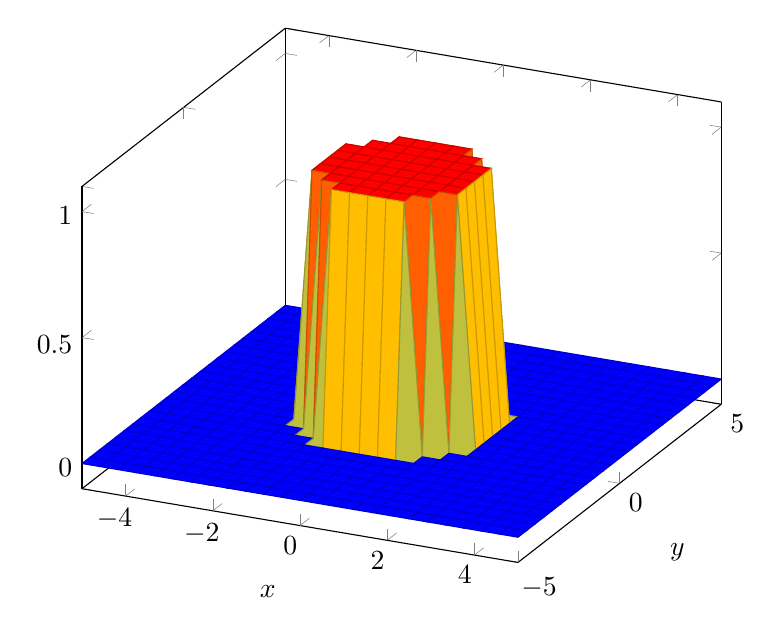
\begin{tikzpicture}

	\begin{axis}[xlabel = $x$, ylabel = $y$, width = 0.8\textwidth]

	\addplot3[surf] {1 * (\R ^ 2 > (x * x + y * y))};

	\end{axis}
	
\end{tikzpicture}
\mimageend

\mimagebegin{ip:3:nb}{Низкочастотный фильтр Баттерворта порядка \bp}
\noindent
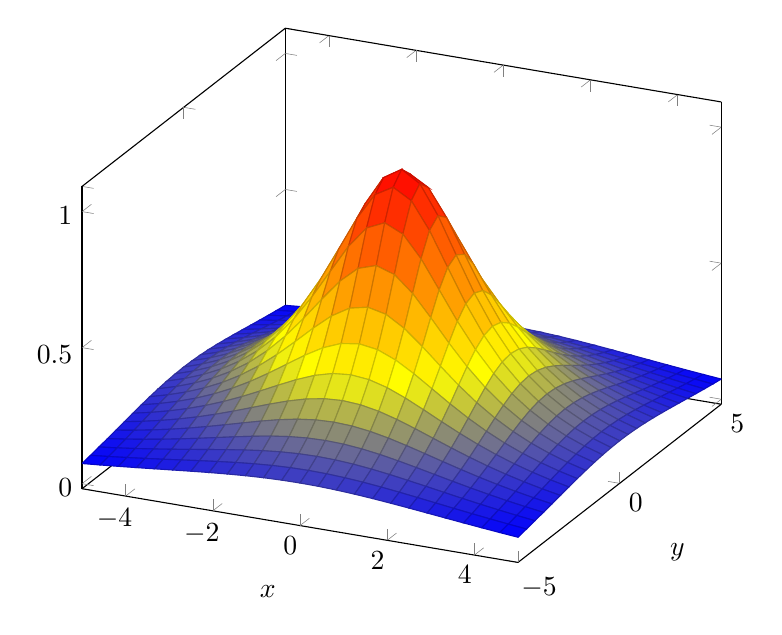
\begin{tikzpicture}

	\begin{axis}[xlabel = $x$, ylabel = $y$, width = 0.8\textwidth]

		\addplot3[surf] {1 / (1 + (sqrt(x * x + y * y) / \R) ^ (2 * \bp))};

	\end{axis}
	
\end{tikzpicture}
\mimageend

\mimagebegin{ip:3:ng}{Низкочастотный фильтр Гаусса}
\noindent
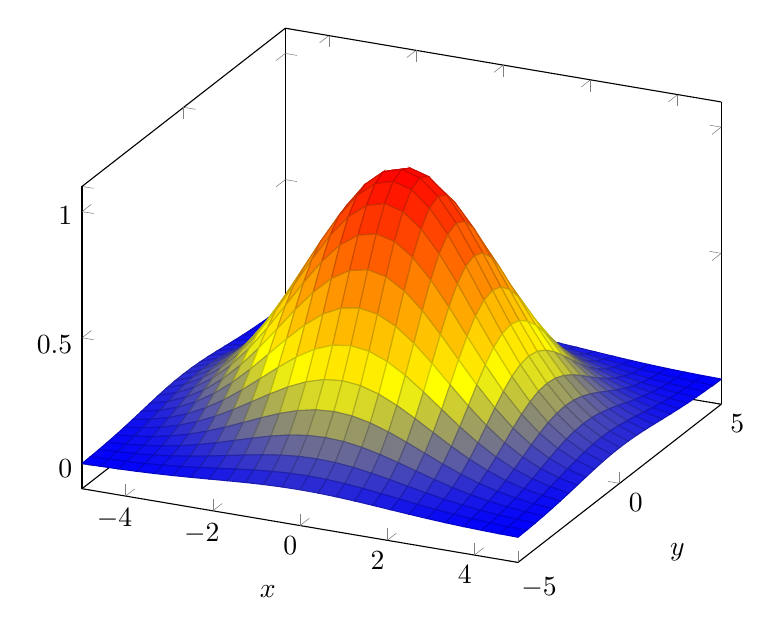
\begin{tikzpicture}

	\begin{axis}[xlabel = $x$, ylabel = $y$, width = 0.8\textwidth]

		\addplot3[surf] {exp(- (x * x + y * y) / (2 * \R ^ 2))};

	\end{axis}
	
\end{tikzpicture}
\mimageend

	\item высокочастотные фильтры.

	Выделяют идеальный высокочастотный фильтр \eqref{ip:3:vi} (рисунок \ref{image:ip:3:vi}), высокочастотный фильтр Баттерворта \eqref{ip:3:vb} (рисунок \ref{image:ip:3:vb}) и высокочастотный фильтр Гаусса \eqref{ip:3:vg} (рисунок \ref{image:ip:3:vg}):
	\begin{gather}
		\label{ip:3:vi} h(u, v) =
		\begin{cases}
			0 ,~ D \le R ^ 2 \\
			1 ,~ D > R ^ 2
		\end{cases} \\
		\label{ip:3:vb} h(u, v) = \dfrac{1}{1 + \left (R / \sqrt{D} \right )^{2n}} \\
		\label{ip:3:vg} h(u, v) = 1 - \exp \left ( \dfrac{- D}{2 R ^ 2} \right ).
	\end{gather}

	Фактически, высокочастотные фильтры суть есть обратные фильтры к своим низкочастотным аналогам.

\mimagebegin{ip:3:vi}{Идеальный высокочастотный фильтр}
\noindent
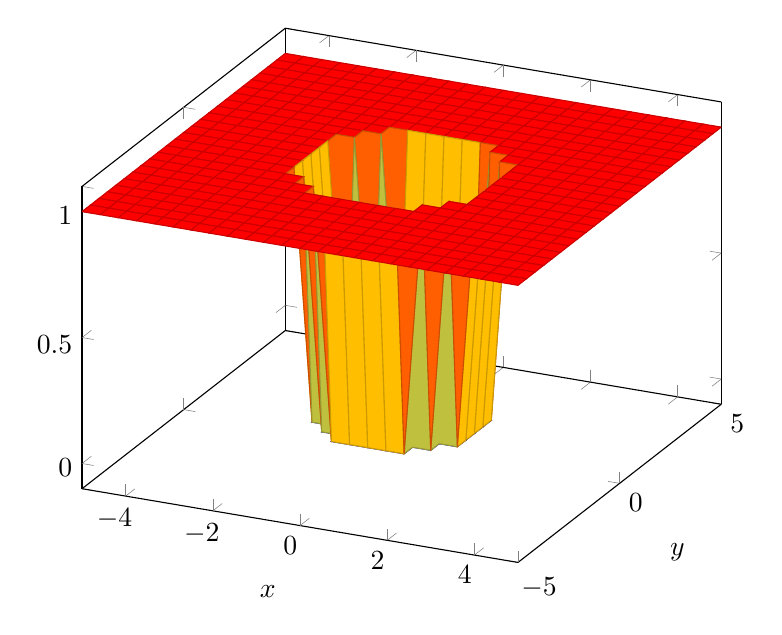
\begin{tikzpicture}

	\begin{axis}[xlabel = $x$, ylabel = $y$, width = 0.8\textwidth]

		\addplot3[surf] {1 * ((x * x + y * y) > \R ^ 2)};

	\end{axis}
	
\end{tikzpicture}
\mimageend

\mimagebegin{ip:3:vb}{Высокочастотный фильтр Баттерворта порядка \bp}
\noindent
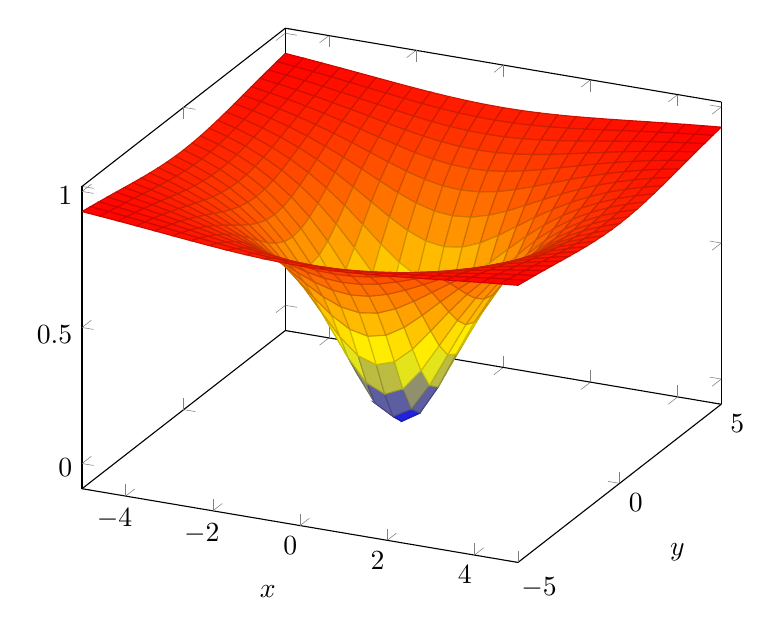
\begin{tikzpicture}

	\begin{axis}[xlabel = $x$, ylabel = $y$, width = 0.8\textwidth]

		\addplot3[surf] {1 / (1 + (\R / sqrt(x * x + y * y)) ^ (2 * \bp))};

	\end{axis}
	
\end{tikzpicture}
\mimageend

\mimagebegin{ip:3:vg}{Высокочастотный фильтр Гаусса}
\noindent
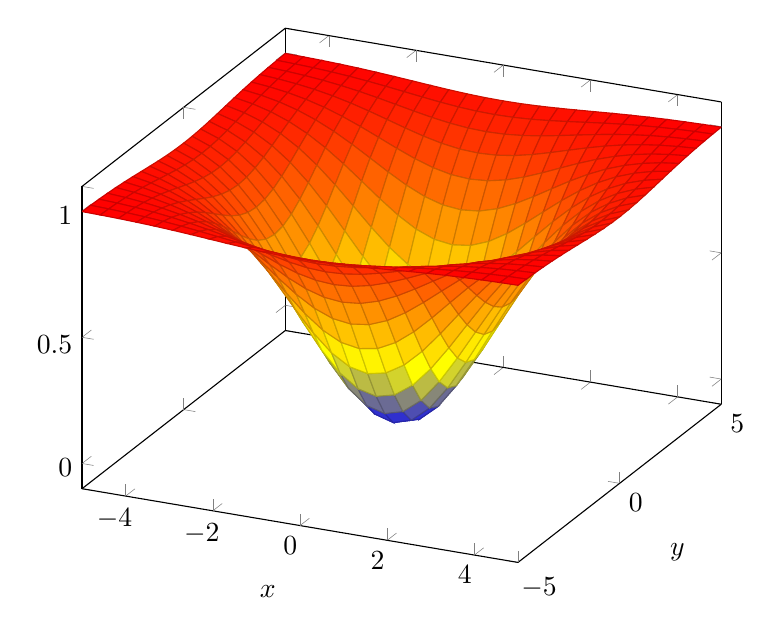
\begin{tikzpicture}

	\begin{axis}[xlabel = $x$, ylabel = $y$, width = 0.8\textwidth]

		\addplot3[surf] {1 - exp(- (x * x + y * y) / (2 * \R ^ 2))};

	\end{axis}
	
\end{tikzpicture}
\mimageend

	\item фильтры, подавляющие периодические шумы.

	Фильтрация периодического шума заключается в минимизации влияния частотных характеристик сигнала в узком диапазоне частот. На изображении - результате преобразования Фурье периодический шум выглядит как ярковыраженная окружность - задача успешной фильтрации, таким образом, заключается в правильном пределении радиуса и ширины границы данной окружности.

	Фильтры, используемые для устранения периодического шума, суть есть режекторные фильтры. Выделяют идеальный режекторный фильтр \eqref{ip:3:ri} (рисунок \ref{image:ip:3:ri}), режекторный фильтр Баттерворта \eqref{ip:3:rb} (рисунок \ref{image:ip:3:rb}) и режекторный фильтр Гаусса \eqref{ip:3:rg}: % (рисунок \ref{image:ip:3:rg}):
	\begin{gather}
		\label{ip:3:ri} h(u, v) =
		\begin{cases}
			1 ,~ D > R_2  ^ 2
			0 ,~ D \ge R_1 ^ 2 ,~ D \le R_2 ^ 2\\
			1 ,~ D < R_1 ^ 2
		\end{cases} \\
		\label{ip:3:rb} h(u, v) = \dfrac{1}{1 + \left (\dfrac{\sqrt{D} (R_2 - R_1)}{D - R_1 ^ 2} \right )^{2n}} \\
		\label{ip:3:rg} h(u, v) = 1 - \exp \left (- \dfrac{1}{2}(\dfrac{D - R_1 ^ 2}{\sqrt{D} (R_2 - R_1)}) ^ 2 \right ),
	\end{gather}

	где $R_2$ и $R_1$ - радиусы внешней и внутренней окружности фильтра (разность $(R_2 - R_1)$ суть есть ширина кольца фильтра).

\def\Runo{2}
\def\Rduo{4}

\mimagebegin{ip:3:ri}{Идеальный режекторный фильтр}
\noindent
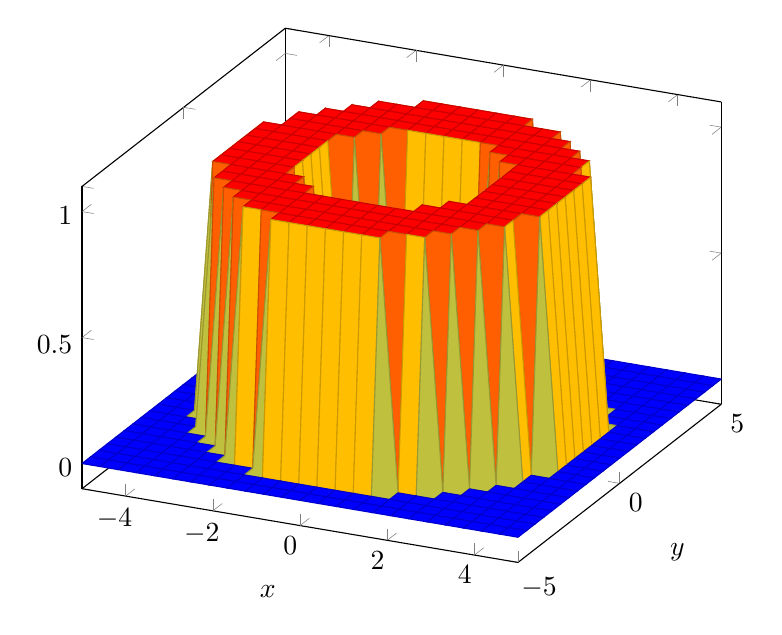
\begin{tikzpicture}

	\begin{axis}[xlabel = $x$, ylabel = $y$, width = 0.8\textwidth]

		\addplot3[surf] {1 * ((x * x + y * y) > \Runo ^ 2) * (\Rduo ^ 2 > (x * x + y * y))};

	\end{axis}
	
\end{tikzpicture}
\mimageend

\mimagebegin{ip:3:rb}{Режекторный фильтр Баттерворта порядка \bp}
\noindent
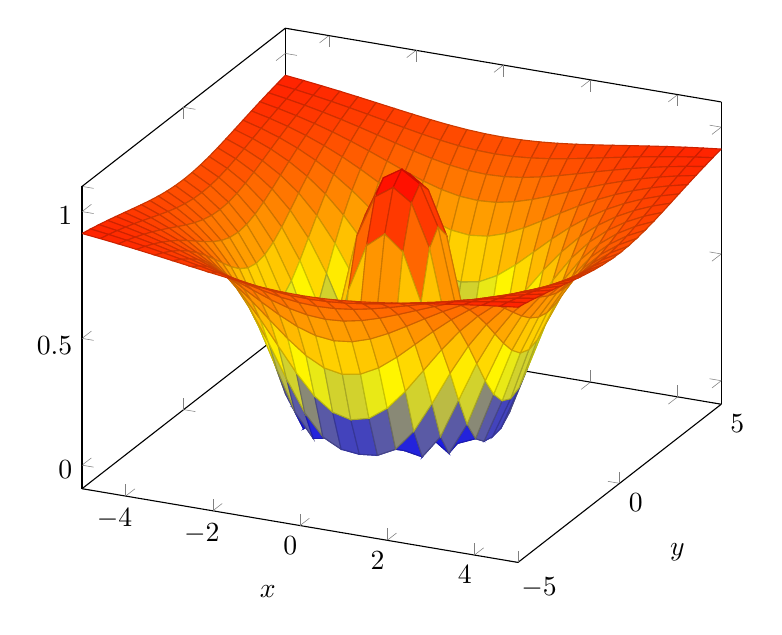
\begin{tikzpicture}

	\begin{axis}[xlabel = $x$, ylabel = $y$, width = 0.8\textwidth]

		\addplot3[surf] {1 / (1 + ((sqrt(x * x + y * y) * (\Rduo - \Runo)) / ((x * x + y * y) - \Runo ^ 2)) ^ (2 * \bp))};

	\end{axis}
	
\end{tikzpicture}
\mimageend

%\mimagebegin{ip:3:rg}{Режекторный фильтр Гаусса}
%\noindent
%\begin{tikzpicture}
%
%	\begin{axis}[xlabel = $x$, ylabel = $y$, width = 0.8\textwidth]
%
%		\addplot3[surf] {1 - exp(- ((((x * x + y * y) - \Runo ^ 2) / (sqrt(x * x + y * y) * (\Rduo - \Runo)))) / 2)};
%
%	\end{axis}
%	
%\end{tikzpicture}
%\mimageend

\end{itemize}

Для конструирования изображения - фильтра средствами библиотеки OpenCV можно воспользоваться функцией \verb|circle()|, прототип которой приведен в листинге \ref{listing:ip:3:circle}.

\mylistingbegin{ip:3:circle}{Отрисовка окружности с помощью функции circle()}
\begin{lstlisting}

void circle(Mat & I, Point center, int R, Scalar color, int thickness);

\end{lstlisting}
\mylistingend

Функция \verb|circle()| отрисовывает окружность радиусом \verb|R| с центром в точке \verb|center| (конструктор класса \verb|Point| обладает двумя параметрами - абсцисса и ордината указываемой точки) на изображении $I$. Цвет окружности задается параметром \verb|color| (класс \verb|Scalar| обладает статическим методом \verb|all()| - фабрикой объектов данного класса - принимающем на свой вход единственный вещественный аргумент - значение яркостей пикселя в каждом из спектральных каналов), ширина окружности - параметром \verb|thickness| (в случае отрицательного значения данного параметра выполняется отрисовка закрашенной окружности).

В некоторых случаях бывает удобно закрасить изображение - фильтр одним цветом (установить все элементы матрицы, описывающей изображение - фильтр, в одно и то же значение), для чего можно воспользоваться методом \verb|setTo()| класса \verb|Mat|. Прототип метода \verb|setTo()| приведен в листинге \ref{listing:ip:3:setto}.

\mylistingbegin{ip:3:setto}{Установ элементов матрицы, описывающей изображение, в одинаковое значение с помощью метода setTo()}
\begin{lstlisting}

Mat & Mat::setTo(Scalar & color);

\end{lstlisting}
\mylistingend

Метод \verb|setTo()| класса \verb|Mat| возвращает описатель нового изображения - результата установа элементов матрицы, описывающей исходное изображение, в одно и то же значение.

\myparagraph{Обработка видеопоследовательностей}

Было бы довольно странно, если бы библиотека OpenCV, решая задачи компьютерного зрения, не предоставляла бы функционал чтения и сохранения видеопоследовательностей. Однако, вопреки всем странностям, таковой функционал в библиотеке OpenCV наличиствует и сосредоточен в классах \verb|VideoCapture| и \verb|VideoWriter|.

\mysubparagraph{Чтение видеопоследовательности}

Библиотека OpenCV предоставляет возможность считывать видеопоследовательности с записывающих устройств (таких как, например, web - камера) или из постоянной памяти (из файлов, расположенных на жестких дисках и прочих носителях).

Считывание видеопоследовательности возможно с помощью объектов класса \verb|VideoCapture|.

Один объект данного класса соответствует одному источнику. Класс \verb|VideoCapture| обладает, кроме всего прочего, методами, прототипы которых приведены в листинге \ref{listing:ip:3:capture}.

\mylistingbegin{ip:3:capture}{Класс VideoCapture, используемый для считывания видеопоследовательностей}
\begin{lstlisting}

VideoCapture::VideoCapture();
bool VideoCapture::open(string fname);
bool VideoCapture::read(Mat & frame);

\end{lstlisting}
\mylistingend

Метод \verb|open()| класса \verb|VideoCapture| позволяет открыть файл, (полный или относительный) путь и имя которого заданы параметром \verb|fname|, на чтение. Метод возвращает \verb|true|, если файл открыть удалось, и \verb|false|, если файл открыть не удалось (например, из-за несовместимого кодека).

Метод \verb|read()| класса \verb|VideoCapture| читает очередной кадр видеопоследовательности и помещает его в матрицу \verb|frame|. Метод возвращает \verb|true|, если кадр считать удалось, и \verb|false|, если кадр считать не удалось (например, из-за достижения конца видеопоследовательности).

Вывод кадров видеопоследовательности производится тем же самым способом, что и вывод обычных изображений. Однако, при выводе кадров видеопоследовательности необходимо помнить о задержке между кадрами. Задержка между кадрами может быть реализована с помощью функции \verb|waitKey()|, одна из перегруженных версий которой обладает параметром, позволяющим указать время (в миллисекундах) ожидания нажатия клавиши.

\mysubparagraph{Сохранение видеопоследовательности}

Библиотека OpenCV позволяет сохранять видеопоследовательность с использованием различных кодеков и контейнеров.

Сохранение видеопоследовательности реализовано библиотекой OpenCV в виде класса \verb|VideoWriter|, прототипы некоторых методов которого приведены в листинге \ref{listing:ip:3:writer}.

\mylistingbegin{ip:3:writer}{Класс VideoWriter, используемый для сохранения видеопоследовательности}
\begin{lstlisting}

VideoWriter::VideoWriter();
bool VideoWriter::open(string fname, int fourcc, double fps, Size size);
void VideoWriter::write(Mat & frame);

\end{lstlisting}
\mylistingend

Метод \verb|open()| класса \verb|VideoWriter| создает (или очищает и открывает на запись) файл - контейнер, тип которого и тип кодека которого указываются с помощью параметра \verb|fourcc| и расширения файла. Путь (абсолютный или относительный) и имя результирующего файла указываются параметром \verb|fname|, частота кадров ((англ.) frame per second; FPS) видеопоследовательности указываются параметром \verb|fps|, размер каждого кадра видеопоследовательности - параметром \verb|size|.

Параметр \verb|fourcc| метода \verb|open()| указывает кодек, используемый для сжатия видеопоследовательности. Для сжатия видеопоследовательности с помощью кодека \verb|MP4| в качестве значения параметра \verb|fourcc| необходимо указать результат вызова макроса \linebreak \verb|CV_FOURCC('M', 'P', '4', 'V')|.

Метод \verb|open()| возвращает \verb|true|, если файл удалось открыть на запись, и \verb|false| - в противном случае.

Метод \verb|write()| класса \verb|VideoWriter| добавляет очередной кадр к видеопоследовательности.

Сохранение видеопоследовательности на диск выполняет деструктор класса \verb|VideoWriter|.

